% !TeX root = ../main.tex

\chapter{系统详细设计与实现}

\section{调度器的实现}

\subsection{决策中心模块的实现}

\subsection{状态转移模块的实现}
调度器中以状态机的设计模型来控制流水线中各个子概念的状态流转。首先以作业为例介绍作业状态机的详细设计。

按照有限状态机的设计理念,我们首先需要确定作业状态机的状态(State)和事件(Event)。
依据需求分析,我们知道作业有:就绪中(Pending)、执行中(Running)、执行成功(Success)、执行失败(Failed)、被跳过(Skipped)和被取消(Canceled)六种状态。
会导致作业状态发生转移的事件包括:触发(Trigger)、重试(Retry)、作业成功(Success)、作业失败(Fail)、作业执行超时(Timeout)、跳过(Skip)、取消(Cancel)。
依据状态机的设计模式,系统中将流水线作业的不同状态封装为类,将引起其状态转移的事件设置为成员方法。图~\ref{fig:作业状态机类图}为作业状态机类图。

\begin{figure}[h]
  \centering
  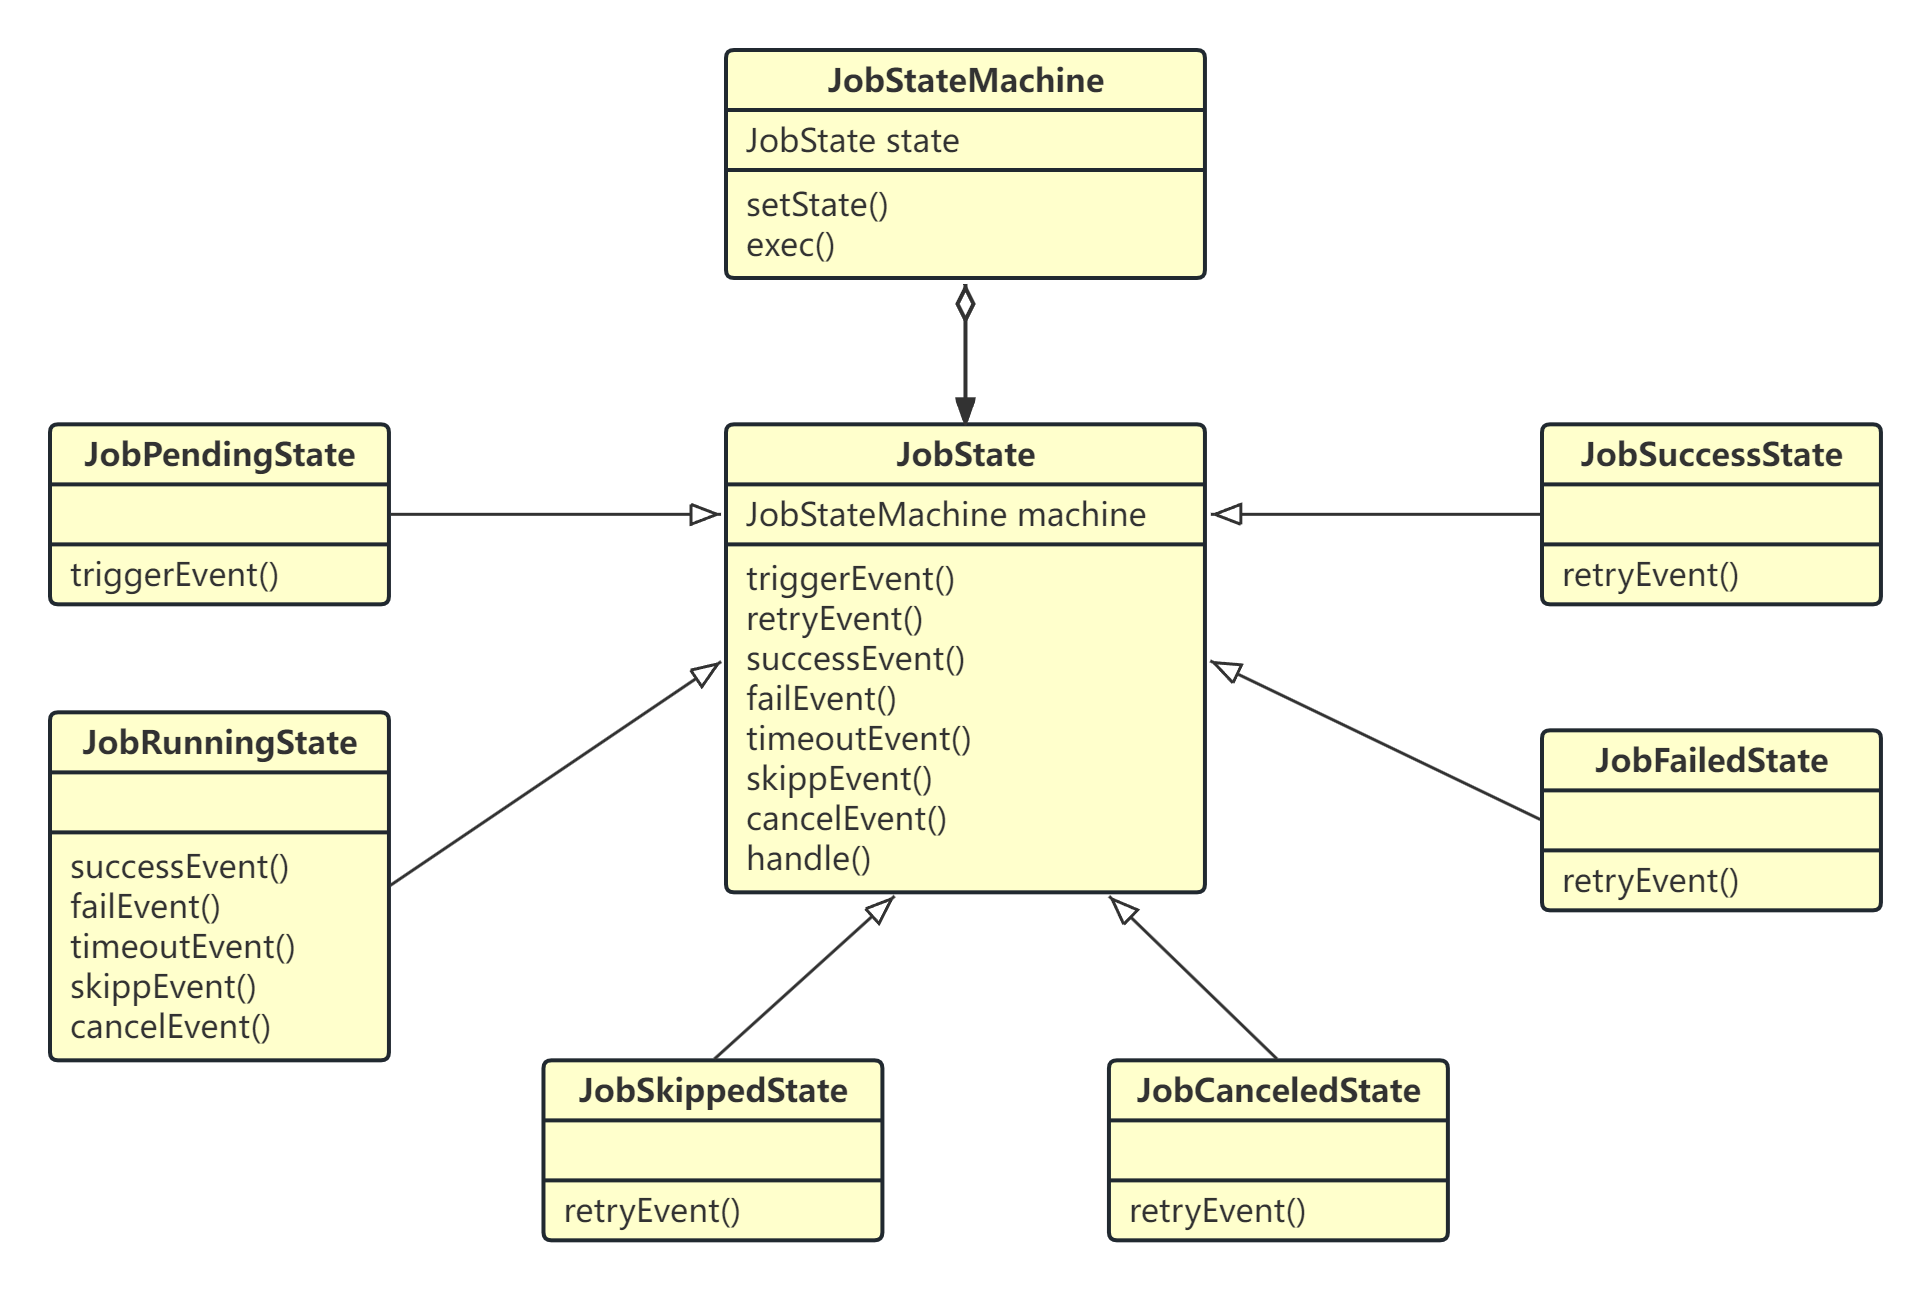
\includegraphics[width=1\textwidth]{作业状态机类图.png}
  \caption{作业状态机类图}
  \label{fig:作业状态机类图}
\end{figure}

当需要进行作业状态转换时,首先创建JobStateMachine实例并设置默认初始状态,然后向exec成员方法中传入当前发生的事件。
其中JobState是作业状态的抽象类,作业中每个具体的状态作为一个JobState的实现类,并从JobState中选择引起其状态转移的事件方法来实现。
例如JobRunningState类实现了JobState中的successEvent、failEvent、timeoutEvent、skippEvent和cancelEvent五个成员方法,这是因为这些事件均能作用于一个正在运行中的作业并且引起其状态改变,
其中successEvent方法会调用父类中持有的实例的JobStateMachine成员的setState方法,将当前状态机的状态设置为成功,并完成一些后续工作,其余事件方法也与之类似。

接下来具体分析作业状态机内部的状态转换:
当一个作业运行实例被创建时其应为就绪中状态,故就绪中(Pending)状态为初始状态,引发其状态改变的事件是触发(triggerEvent),这个触发事件是由决策中心经过决策逻辑发出的,并不只是用户的动触发行为,
一旦作业被成功触发,其状态则改变为运行中(Running);如果该作业被设定为需要人工审核才能触发,则审核通过事件(reviewApproveEvent)将会将状态改变为运行中(Running),审核驳回事件(reviewRejectEvent)将会将状态改变为失败(Failed)。
当作业处于运行中时,调度器可能会收到来自两方面的信号,其一是执行器所通知的作业执行状态,包括作业执行成功(successEvent)、执行失败(failEvent)和执行超时(timeoutEvent),
其中执行成功会使得作业状态机变为执行成功状态(Success),执行失败和执行超时都会变为执行失败状态(Failed);
其二是CI-Service所通知的用户人工干预命令,包括取消作业(cancelEvent)和跳过(skipEvent)作业,这两种事件会立即使得作业状态机变为取消(Canceled)和跳过(Skipped)状态。
以上两种信号均由决策中心先收到信号并统一处理决策后再转发给状态机,这样做可以统一外界信号的入口,降低其他模块与调度器间的耦合。
当处于运行中的作业进入终态后,作业仍然可以通过重试事件(retryEvent)来重新进入运行中的状态。
至于当前的作业是否满足触发该事件的条件,或者是否需要人工审核,由决策中心统一处理后发出信号,状态机不做额外的业务逻辑判断。

图~\ref{fig:流水线作业状态图}展示了作业状态机的状态流转。

\begin{figure}[h]
  \centering
  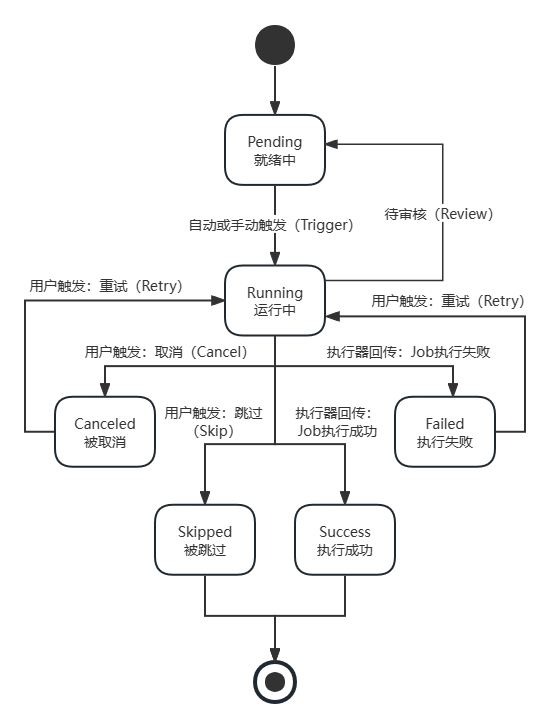
\includegraphics[width=0.7\textwidth]{流水线作业状态图.png}
  \caption{流水线作业状态图}
  \label{fig:流水线作业状态图}
\end{figure}



\subsection{作业管理模块的实现}





\subsection{二级节标题}

\subsubsection{三级节标题}

\paragraph{四级节标题}

\subparagraph{五级节标题}
